\documentclass[a4paper,twocolumn,11pt]{memoir}
\usepackage[a4paper]{geometry}
\geometry{verbose,tmargin=1.5cm,bmargin=1.5cm,lmargin=1cm,rmargin=1cm}

\setlength{\parskip}{\smallskipamount}
\setlength{\parindent}{0pt}

\usepackage{fontspec}
\defaultfontfeatures{Ligatures=TeX}
\setmainfont{Linux Libertine O}

\usepackage{hyperref}
\usepackage{url}
\usepackage{xcolor}

\usepackage{amsmath}
\usepackage{amssymb}
\usepackage{braket}

\usepackage{minted}
\newminted{fortran}{breaklines,fontsize=\footnotesize}
\newminted{python}{breaklines,fontsize=\footnotesize}

\definecolor{mintedbg}{rgb}{0.95,0.95,0.95}
\usepackage{mdframed}

\newcommand{\ffrLFDFT}{{\texttt{ffr-LFDFT}}\,}
\newcommand{\ffrmain}{{\texttt{ffr\_LFDFT.x}}\,}


\begin{document}


\title{Implementation Notes of \ffrLFDFT}
\author{Fadjar Fathurrahman}
%\date{}
\maketitle

\newpage

\tableofcontents

\chapter{Lagrange functions in one dimension}


\section{Introduction}

There are various ways to derive what will be referred to as
Lagrange basis functions (LBFs) or Lagrange functions (LFs) below.
In some references, they are also referred to as discrete variable
representation (DVR) basis functions, especially in papers by Tuckerman's
research group [references needed].

In summary, this is the parameters that are needed to specify a specific
LBFs:
\begin{itemize}

\item For periodic and cluster/box LBFs we need to specify:
\begin{itemize}
\item number of basis functions $N$
\item two end points $a$ and $b$
\end{itemize}

\item For sinc LBFs, we need to specify:
\begin{itemize}
\item number of basis functions $N$
\item grid spacing $h$
\end{itemize}

\end{itemize}


\section{Implementation}

Currently, there is only special module to handle global variables related
to 1D LFs. However, there is a special module to handle 3D LFs, namely
the module \texttt{m\_LF3d} defined in file \texttt{m\_LF3d.f90}.
The relevant global variables for our current discussion are the following.
\begin{fortrancode}
INTEGER :: LF3d_NN(3)
REAL(8) :: LF3d_LL(3)
REAL(8) :: LF3d_AA(3), LF3d_BB(3)
REAL(8) :: LF3d_hh(3)
\end{fortrancode}
Note that, these arrays are of size 3, for each $x$, $y$, and $z$ component.
We will restrict ourself to 1D, and will take only the first element, i.e. the
$x$ direction.
The grid points are stored in array:
\begin{fortrancode}
REAL(8), ALLOCATABLE :: LF3d_grid_x(:)
\end{fortrancode}

In the actual code, if there is no name-clash (i.e. no two or more variables with the
same name), we usually use the aliases for these global variables, e.g.:
\begin{fortrancode}
USE m_LF3d, ONLY : NN => LF3d_NN, hh => LF3d_hh
\end{fortrancode}

The relevant subroutines to initialize the grid points for each LFs:
\begin{itemize}
\item \texttt{init\_grid\_1d\_p()}
\item \texttt{init\_grid\_1d\_c()}
\item \texttt{init\_grid\_1d\_sinc()}
\end{itemize}



\section{Initializing grid points for LFs}

The following code fragments initializes 1D periodic LFs:
\begin{fortrancode}
USE m_LF3d, ONLY : grid_x => LF3d_grid_x
IMPLICIT NONE
INTEGER :: N, i
REAL(8) :: L
! Initialize the basis functions
ALLOCATE( grid_x(N) )
CALL init_grid_1d_p( N, -0.5d0*L, 0.5d0*L, grid_x )
WRITE(*,'(1x,A,I5)') 'N = ', N
WRITE(*,'(1x,A,F18.10)') 'L = ', L
WRITE(*,'(1x,A,F18.10)') 'Grid spacing = ', grid_x(2) - grid_x(1)
WRITE(*,*) 'Grid points for periodic LF'
DO i = 1,N
  WRITE(*,'(1x,I5,F18.10)') i, grid_x(i)
ENDDO
DEALLOCATE( grid_x )
\end{fortrancode}

A complete example code can be found in file \texttt{tests/init/ex\_init\_1d.f90}.


\section{Plotting the basis functions}

The relevant subroutines used for this purpose are as follows.
\begin{itemize}
\item \texttt{eval\_LF1d\_p()}
\item \texttt{eval\_LF1d\_c()}
\item \texttt{eval\_LF1d\_sinc()}
\end{itemize}

Plots of periodic, cluster/box, and sinc LFs are
shown in Figure \ref{fig:LF1d_p_5}, \ref{fig:LF1d_c_5}, and
\ref{fig:LF1d_sinc_5} respectively.

\begin{figure}[h]
{\centering
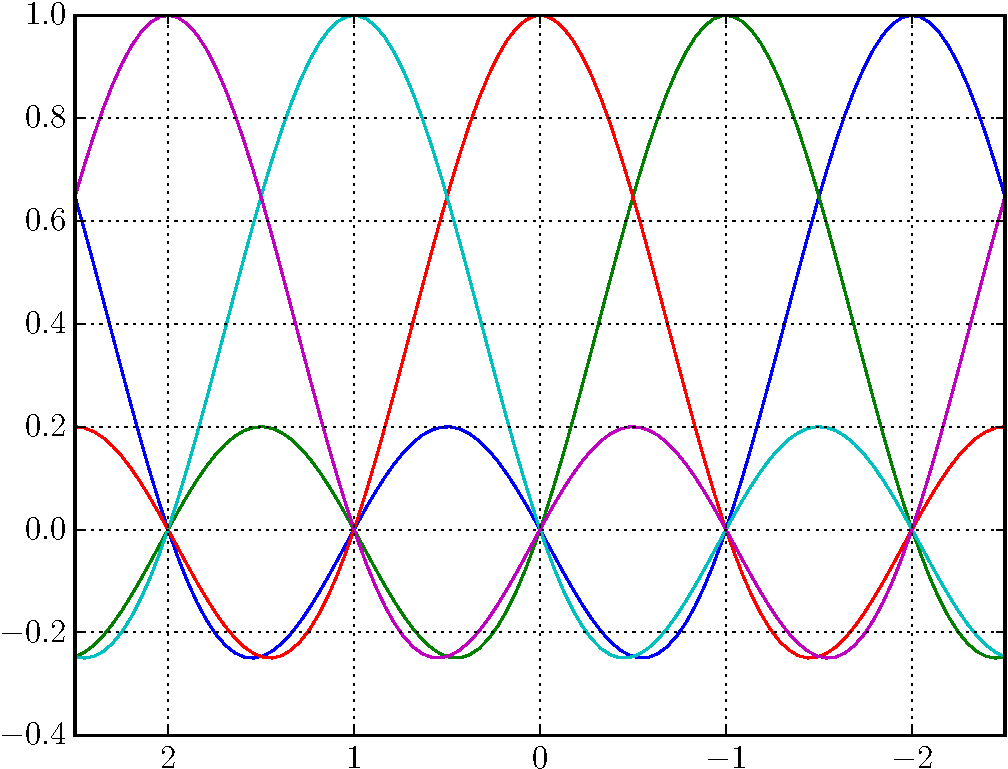
\includegraphics[width=0.5\textwidth]{../../tests/plot_1d/LF1d_p.pdf}
\par}
\caption{Periodic LF}\label{fig:LF1d_p_5}
\end{figure}

An example program which can produce plot data for these figures can be
found in \texttt{tests/plot\_1d/ex\_plot\_1d.f90}.

\begin{figure}[h]
{\centering
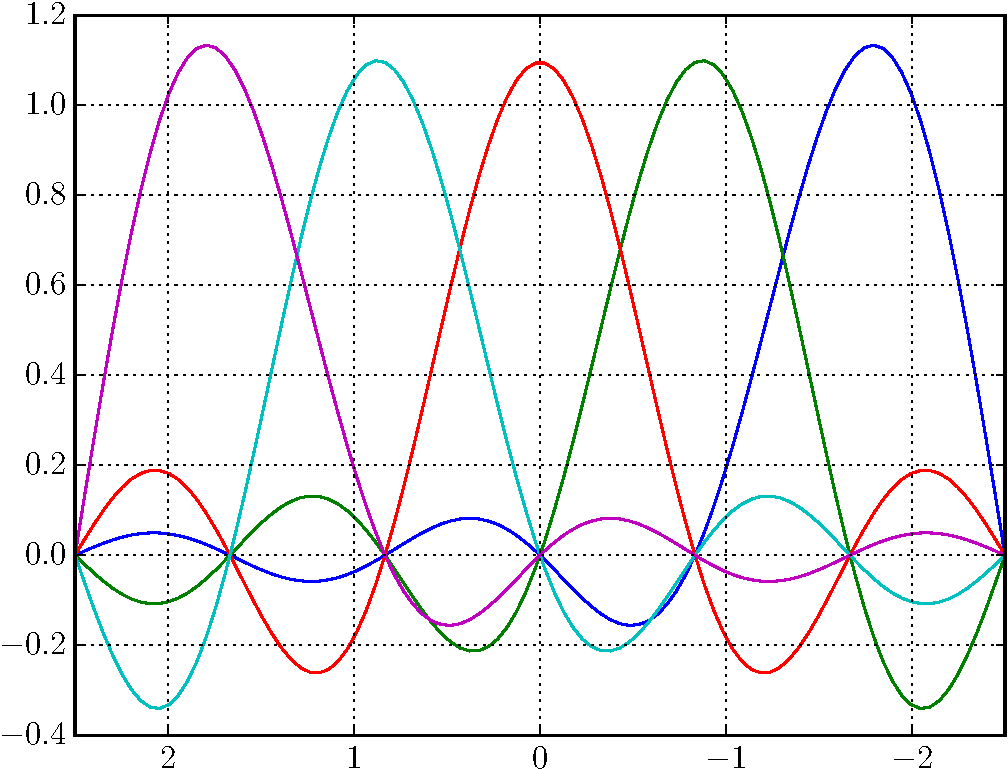
\includegraphics[width=0.5\textwidth]{../../tests/plot_1d/LF1d_c.pdf}
\par}
\caption{Cluster/box LF}\label{fig:LF1d_c_5}
\end{figure}

The following Python script were used to plot the resulting data:
\begin{pythoncode}
import numpy as np
import matplotlib.pyplot as plt
import os
from matplotlib import rc
rc('font',**{'family':'serif', 'size':16})
rc('text', usetex=True)
types = ['sinc', 'c', 'p']
NBASIS = 5
for t in types:
    dat1 = np.loadtxt('LF1d_' + t + '.dat')
    plt.clf()
    for ibf in range(1,NBASIS+1):
        plt.plot( dat1[:,0], dat1[:,ibf] )
    plt.xlim( dat1[-1,0], dat1[0,0] )
    plt.grid()
    FIPLOT = 'LF1d_' + t + '.pdf'
    plt.savefig(FIPLOT)
    os.system('pdfcrop ' + FIPLOT + ' ' + FIPLOT)
\end{pythoncode}

\begin{figure}[h]
{\centering
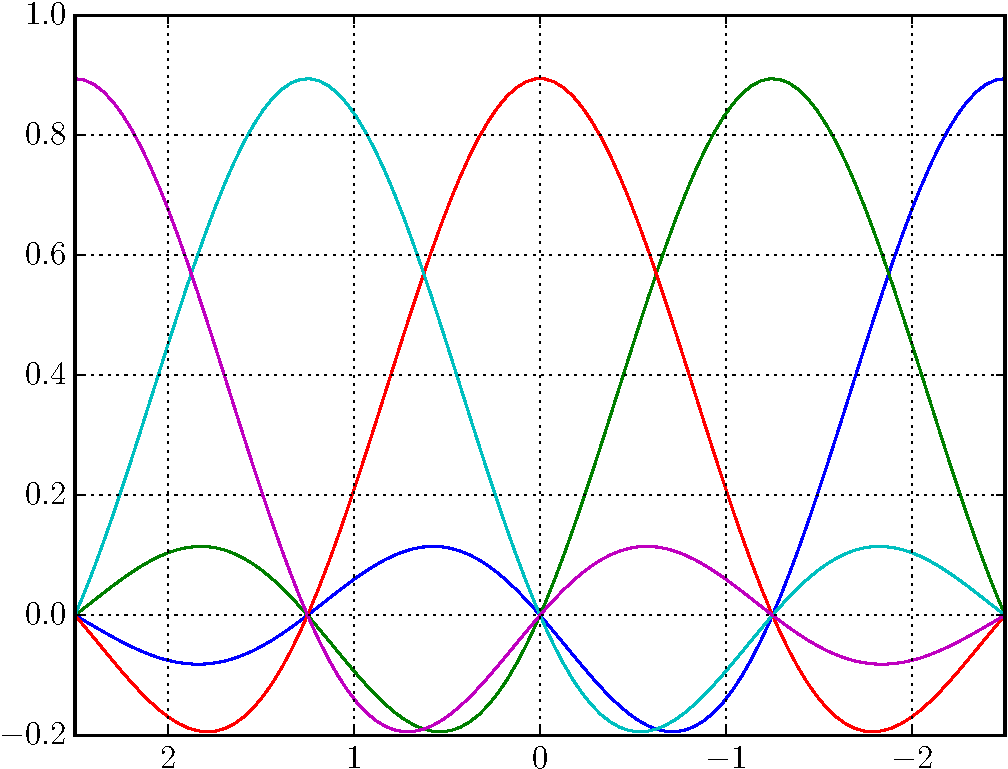
\includegraphics[width=0.5\textwidth]{../../tests/plot_1d/LF1d_sinc.pdf}
\par}
\caption{Sinc LF}\label{fig:LF1d_sinc_5}
\end{figure}


\section{Basis function expansion}

We can expand any "appropriate" function $f(x)$ using LFs:
\begin{equation}
f(x) = \sum_{i}^{N} c_{i} \varphi_{i}(x)
\end{equation}
with $c_{i} = f(x_{i}) \sqrt{\Delta}$

also can use notation $h = \Delta = L/N$

Directory: \texttt{expand\_1d\_p}





\section{Approximating integrals}

Integral can be approximated as
\begin{equation}
\int f(x)\,\mathrm{d}x \approx \Delta x \sum_{i} f(x_{i})
\end{equation}

Directory: \texttt{integ\_1d}


\chapter{Solving Schrodinger equation in 1D}

Minimization method

Using diagonalization
- CG diagonalization
- Davidson
- LOBPCG


\chapter{Lagrange functions in three dimension}

Linear grid 


\appendix

\chapter{HGH pseudopotential}

\section{Implementation}

\chapter{Interpolation with \texttt{bspline}}

\texttt{bspline} library by Jacob Williams.

\section{Interpolation in 1D}


\section{Interpolation in 3D}

Determines the parameters of a function that interpolates
the three-dimensional gridded data

$$ [x(i),y(j),z(k),\mathrm{fcn}(i,j,k)] ~\mathrm{for}~
   i=1,..,n_x ~\mathrm{and}~ j=1,..,n_y, ~\mathrm{and}~ k=1,..,n_z $$

The interpolating function and
its derivatives may subsequently be evaluated by the function
[[db3val]].

The interpolating function is a piecewise polynomial function
represented as a tensor product of one-dimensional b-splines. the
form of this function is

$$ s(x,y,z) = \sum_{i=1}^{n_x} \sum_{j=1}^{n_y} \sum_{k=1}^{n_z}
              a_{ijk} u_i(x) v_j(y) w_k(z) $$

where the functions \(u_i\), \(v_j\), and \(w_k\) are one-dimensional b-
spline basis functions. the coefficients \(a_{ijk}\) are chosen so that:

$$ s(x(i),y(j),z(k)) = \mathrm{fcn}(i,j,k)
   ~\mathrm{for}~ i=1,..,n_x , j=1,..,n_y , k=1,..,n_z $$

Note that for fixed values of \(y\) and \(z\) \(s(x,y,z)\) is a piecewise
polynomial function of \(x\) alone, for fixed values of \(x\) and \(z\) \(s(x,y,z)\)
is a piecewise polynomial function of \(y\) alone, and for fixed
values of \(x\) and \(y\) \(s(x,y,z)\) is a function of \(z\) alone. in one
dimension a piecewise polynomial may be created by partitioning a
given interval into subintervals and defining a distinct polynomial
piece on each one. the points where adjacent subintervals meet are
called knots. each of the functions \(u_i\), \(v_j\), and \(w_k\) above is a
piecewise polynomial.

Users of [[db3ink]] choose the order (degree+1) of the polynomial
pieces used to define the piecewise polynomial in each of the \(x\), \(y\),
and \(z\) directions (`kx`, `ky`, and `kz`). users also may define their own
knot sequence in \(x\), \(y\), \(z\) separately (`tx`, `ty`, and `tz`). if `iflag=0`,
however, [[db3ink]] will choose sequences of knots that result in a
piecewise polynomial interpolant with `kx-2` continuous partial
derivatives in \(x\), `ky-2` continuous partial derivatives in \(y\), and `kz-2`
continuous partial derivatives in \(z\). (`kx` knots are taken near
each endpoint in \(x\), not-a-knot end conditions are used, and the
remaining knots are placed at data points if `kx` is even or at
midpoints between data points if `kx` is odd. the \(y\) and \(z\) directions
are treated similarly.)
After a call to [[db3ink]], all information necessary to define the
interpolating function are contained in the parameters `nx`, `ny`, `nz`,
`kx`, `ky`, `kz`, `tx`, `ty`, `tz`, and `bcoef`. these quantities should not be
altered until after the last call of the evaluation routine [[db3val]].


\begin{fortrancode}
pure subroutine db3ink(x,nx,y,ny,z,nz,fcn,kx,ky,kz,iknot,tx,ty,tz,bcoef,iflag)

  integer,intent(in) :: nx !! number of \(x\) abcissae ( $ \ge 3 $ )
  integer,intent(in) :: ny !! number of \(y\) abcissae ( $ \ge 3 $ )
  integer,intent(in) :: nz !! number of \(z\) abcissae ( $ \ge 3 $ )

  integer,intent(in) :: kx
  !! The order of spline pieces in \(x\) ( \( 2 \le k_x < n_x \) )
  !! (order = polynomial degree + 1)

  integer,intent(in) :: ky
  !! The order of spline pieces in \(y\) ( \( 2 \le k_y < n_y \) )
  !! (order = polynomial degree + 1)

  integer,intent(in) :: kz
  !! the order of spline pieces in \(z\) ( \( 2 \le k_z < n_z \) )
  !! (order = polynomial degree + 1)

  real(8),dimension(:),intent(in) :: x
  !! `(nx)` array of $x$ abcissae. must be strictly increasing.

  real(8),dimension(:),intent(in) :: y
  !! `(ny)` array of $y$ abcissae. must be strictly increasing.

  real(8),dimension(:),intent(in) :: z
  !! `(nz)` array of $z$ abcissae. must be strictly increasing.

  real(8),dimension(:,:,:),intent(in) :: fcn
  !! `(nx,ny,nz)` matrix of function values to interpolate. `fcn(i,j,k)` should
  !! contain the function value at the point (`x(i)`,`y(j)`,`z(k)`)

  integer,intent(in) :: iknot
  !! knot sequence flag:
  !!
  !! * 0 = knot sequence chosen by [[db3ink]].
  !! * 1 = knot sequence chosen by user.

  real(8),dimension(:),intent(inout) :: tx
  !! The `(nx+kx)` knots in the \(x\) direction for the spline interpolant.
  !!
  !! * If `iknot=0` these are chosen by [[db3ink]].
  !! * If `iknot=1` these are specified by the user.
  !!
  !! Must be non-decreasing.

  real(8),dimension(:),intent(inout) :: ty
  !! The `(ny+ky)` knots in the \(y\) direction for the spline interpolant.
  !!
  !! * If `iknot=0` these are chosen by [[db3ink]].
  !! * If `iknot=1` these are specified by the user.
  !!
  !! Must be non-decreasing.

  real(8),dimension(:),intent(inout) :: tz
  !! The `(nz+kz)` knots in the $z$ direction for the spline interpolant.
  !!
  !! * If `iknot=0` these are chosen by [[db3ink]].
  !! * If `iknot=1` these are specified by the user.
  !!
  !! Must be non-decreasing.

  real(8),dimension(:,:,:),intent(out) :: bcoef
  !! `(nx,ny,nz)` matrix of coefficients of the b-spline interpolant.

  integer,intent(out) :: iflag
  !! *  0 = successful execution.
  !! *  2 = `iknot` out of range.
  !! *  3 = `nx` out of range.
  !! *  4 = `kx` out of range.
  !! *  5 = `x` not strictly increasing.
  !! *  6 = `tx` not non-decreasing.
  !! *  7 = `ny` out of range.
  !! *  8 = `ky` out of range.
  !! *  9 = `y` not strictly increasing.
  !! * 10 = `ty` not non-decreasing.
  !! * 11 = `nz` out of range.
  !! * 12 = `kz` out of range.
  !! * 13 = `z` not strictly increasing.
  !! * 14 = `ty` not non-decreasing.
  !! * 700 = `size(x) ` $\ne$ `size(fcn,1)`
  !! * 701 = `size(y) ` $\ne$ `size(fcn,2)`
  !! * 702 = `size(z) ` $\ne$ `size(fcn,3)`
  !! * 706 = `size(x) ` $\ne$ `nx`
  !! * 707 = `size(y) ` $\ne$ `ny`
  !! * 708 = `size(z) ` $\ne$ `nz`
  !! * 712 = `size(tx)` $\ne$ `nx+kx`
  !! * 713 = `size(ty)` $\ne$ `ny+ky`
  !! * 714 = `size(tz)` $\ne$ `nz+kz`
  !! * 800 = `size(x) ` $\ne$ `size(bcoef,1)`
  !! * 801 = `size(y) ` $\ne$ `size(bcoef,2)`
  !! * 802 = `size(z) ` $\ne$ `size(bcoef,3)`
\end{fortrancode}

\chapter{Fast Fourier Transform using \texttt{fftw3}}

3D FFT

C code

Fortran code


\end{document}
